\documentclass[12pt]{article}

\usepackage{fullpage}
\usepackage{graphicx, rotating, booktabs} 
\usepackage{times} 
\usepackage{natbib} 
\usepackage{indentfirst} 
\usepackage{setspace}
\usepackage{grffile} 
\usepackage{hyperref}
\usepackage{adjustbox}
\usepackage{amsmath}
\usepackage{siunitx}
\setcitestyle{aysep{}}


\singlespace
\title{\textbf{Appendix: Democracy and Alliance Treaty Depth}}
\author{}
\date{}

\bibliographystyle{apsr}

\begin{document}

\maketitle 

\doublespace 

This appendix contains a series of robustness checks for the findings in the manuscript. 
In the first section, I examine results with an alternative measure of democracy when the alliance formed: the proportion of democracies in the alliance. 
Then I look at results from two alternative measures of treaty depth.
In the third section, I use hurdle models to   
Last, I consider how uncertainty in the latent treaty depth measure affects my inferences. 


\section{Proportion of Democracies}


The proportion of democracies in the alliance is an alternative measure of how much heft democracies have in negotiations \cite{Chibaetal2015}.  
Rather than the POLITY scores of the most capable alliance member, this variable is the share of alliance members with a POLITY score greater than 5, which is a common threshold for democracy. 
I expect that the proportion measure should lead to similar inferences about the connection between democracy and alliance treaty depth.

First, the descriptive statistics for the proportion of democracies across treaty depth and unconditional military support are as expected. 
\autoref{fig:democ-prop-combo} shows the average proportion of democracies in four types of alliances. 
Deep, conditional alliances have the highest average proportion of democratic members, although it is not much higher than the shallow and conditional average.  


\begin{figure}
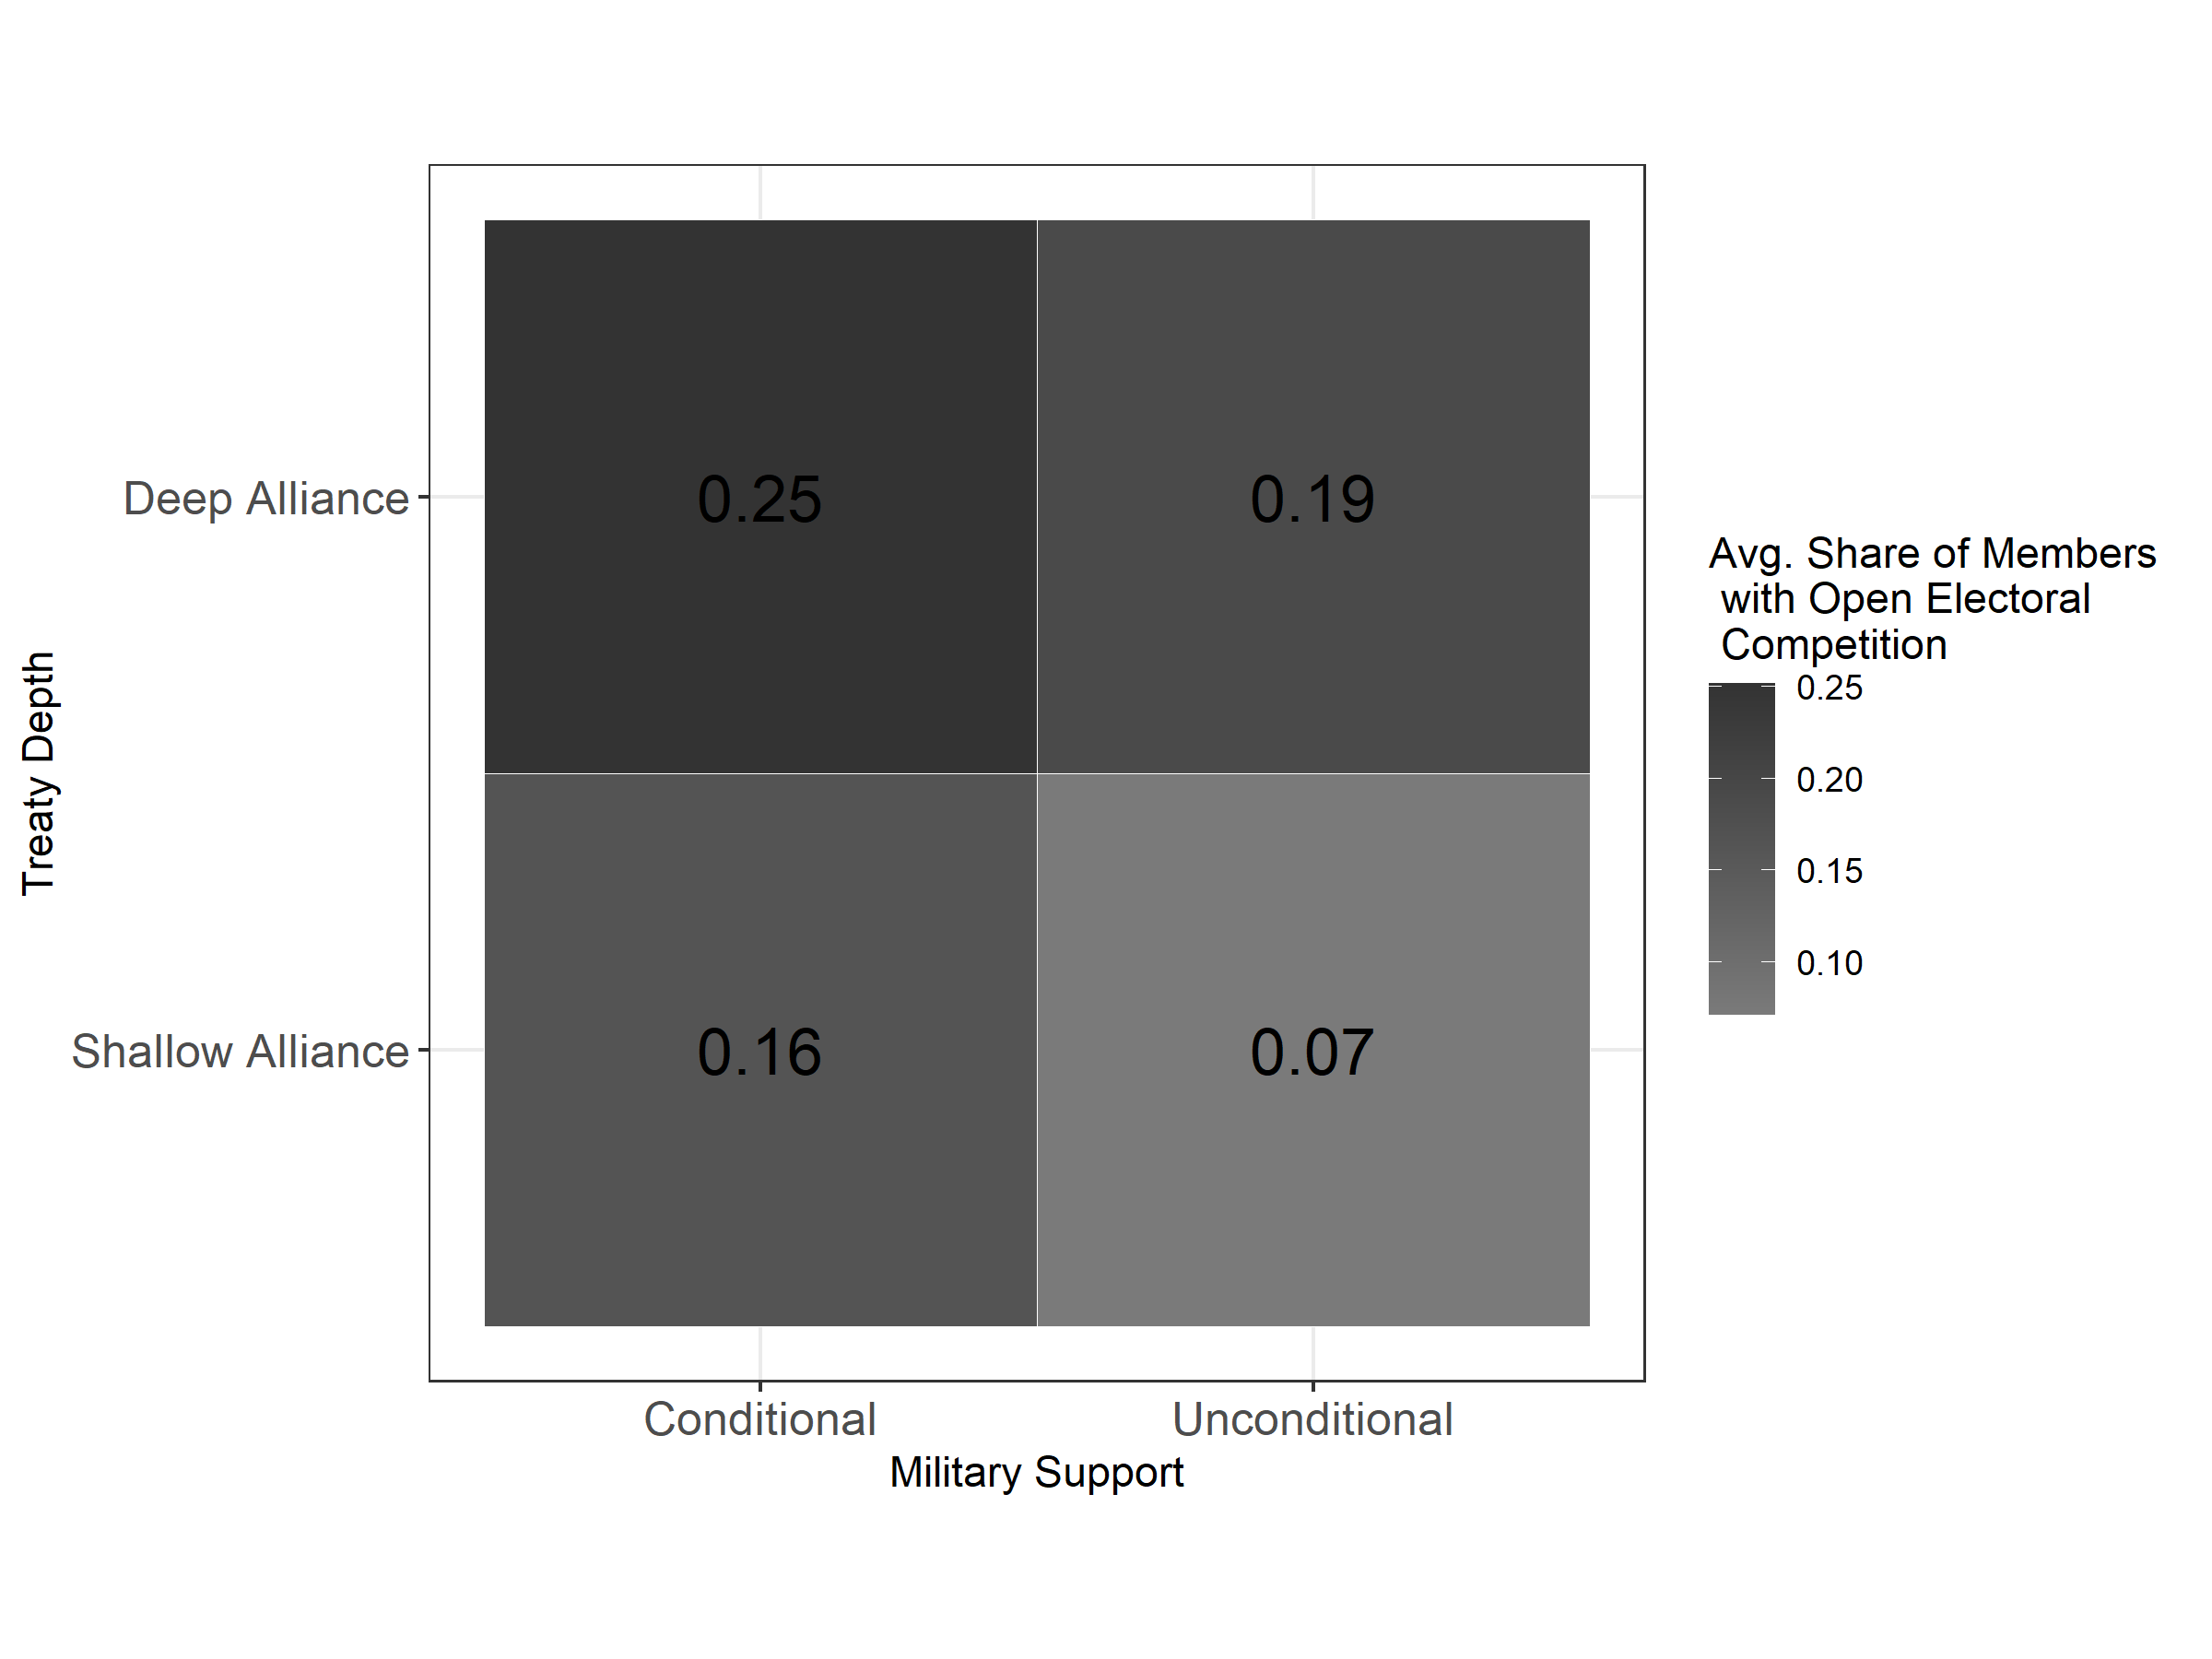
\includegraphics[width=.95\textwidth]{democ-prop-combo.png}  
\caption{Average proportion of democratic members in four groups of alliances. Alliances are grouped based on treaty depth and unconditional military support.}
\label{fig:democ-prop-combo}
\end{figure}


In \autoref{tab:separate-models-prop}, I summarize the results of separate models, which find weak associations for depth and unconditional military support. 
These results are weaker than expected, which may reflect differences in influence, or the competing effects of democratic institutions I identified in the paper. 


\begin{table}[!htbp] \centering 
  \caption{} 
  \label{tab:separate-models-prop} 
\begin{tabular}{@{\extracolsep{5pt}}lcc} 
\\[-1.8ex]\hline 
\hline \\[-1.8ex] 
 & \multicolumn{2}{c}{\textit{Dependent variable:}} \\ 
\cline{2-3} 
\\[-1.8ex] & Latent Depth (rescaled) & Unconditional Military Support \\ 
\\[-1.8ex] & \textit{beta} & \textit{probit} \\ 
\\[-1.8ex] & (1) & (2)\\ 
\hline \\[-1.8ex] 
 Proportion of Democracies & 0.125 & $-$0.516 \\ 
  & ($-$0.334, 0.583) & ($-$1.176, 0.145) \\ 
  Foreign Policy Concessions & $-$0.092 & 0.006 \\ 
  & ($-$0.246, 0.061) & ($-$0.214, 0.227) \\ 
  Number of Members & 0.024$^{}$ & $-$0.031 \\ 
  & ($-$0.002, 0.050) & ($-$0.077, 0.015) \\ 
  Wartime Alliance & $-$0.275 & $-$0.980$^{}$ \\ 
  & ($-$0.624, 0.074) & ($-$1.597, $-$0.363) \\ 
  Asymmetric Obligations & 0.283$^{}$ & 0.038 \\ 
  & ($-$0.053, 0.619) & ($-$0.456, 0.532) \\ 
  Asymmetric Capability & 0.346 & 0.600 \\ 
  & ($-$0.123, 0.815) & ($-$0.269, 1.468) \\ 
  Non-Major Only & 0.253 & 1.093$^{}$ \\ 
  & ($-$0.254, 0.760) & (0.209, 1.977) \\ 
  Average Threat & 1.101$^{}$ & 1.645$^{}$ \\ 
  & (0.238, 1.965) & (0.328, 2.961) \\ 
  Foreign Policy Disagreement & 0.117 & 0.384 \\ 
  & ($-$0.339, 0.573) & ($-$0.312, 1.079) \\ 
  Start Year & 0.004$^{}$ & 0.015$^{}$ \\ 
  & (0.001, 0.008) & (0.010, 0.021) \\ 
  Constant & $-$9.468$^{}$ & $-$31.466$^{}$ \\ 
  & ($-$16.269, $-$2.668) & ($-$42.952, $-$19.979) \\ 
 \hline \\[-1.8ex] 
Observations & 277 & 277 \\ 
Log Likelihood & 52.250 & $-$132.053 \\ 
\hline 
\hline \\[-1.8ex] 
\textit{Note:}  & \multicolumn{2}{r}{95\% Confidence Intervals in Parentheses.} \\ 
\end{tabular} 
\end{table} 



Results from a generalized joint regression model of treaty depth and unconditional military support as a function of the proportion of democracies match the findings in the paper.
In \autoref{fig:results-prop}, there is a no substantive association between the proportion of democracies in an alliance and the probability of unconditional military support. 
Alliances between democracies are more likely to have high treaty depth, however. 
Therefore, I find little evidence that democracies are more likely to form alliances with conditional obligations, but I do find a positive relationship between democratic alliance membership and treaty depth. 


\begin{figure}
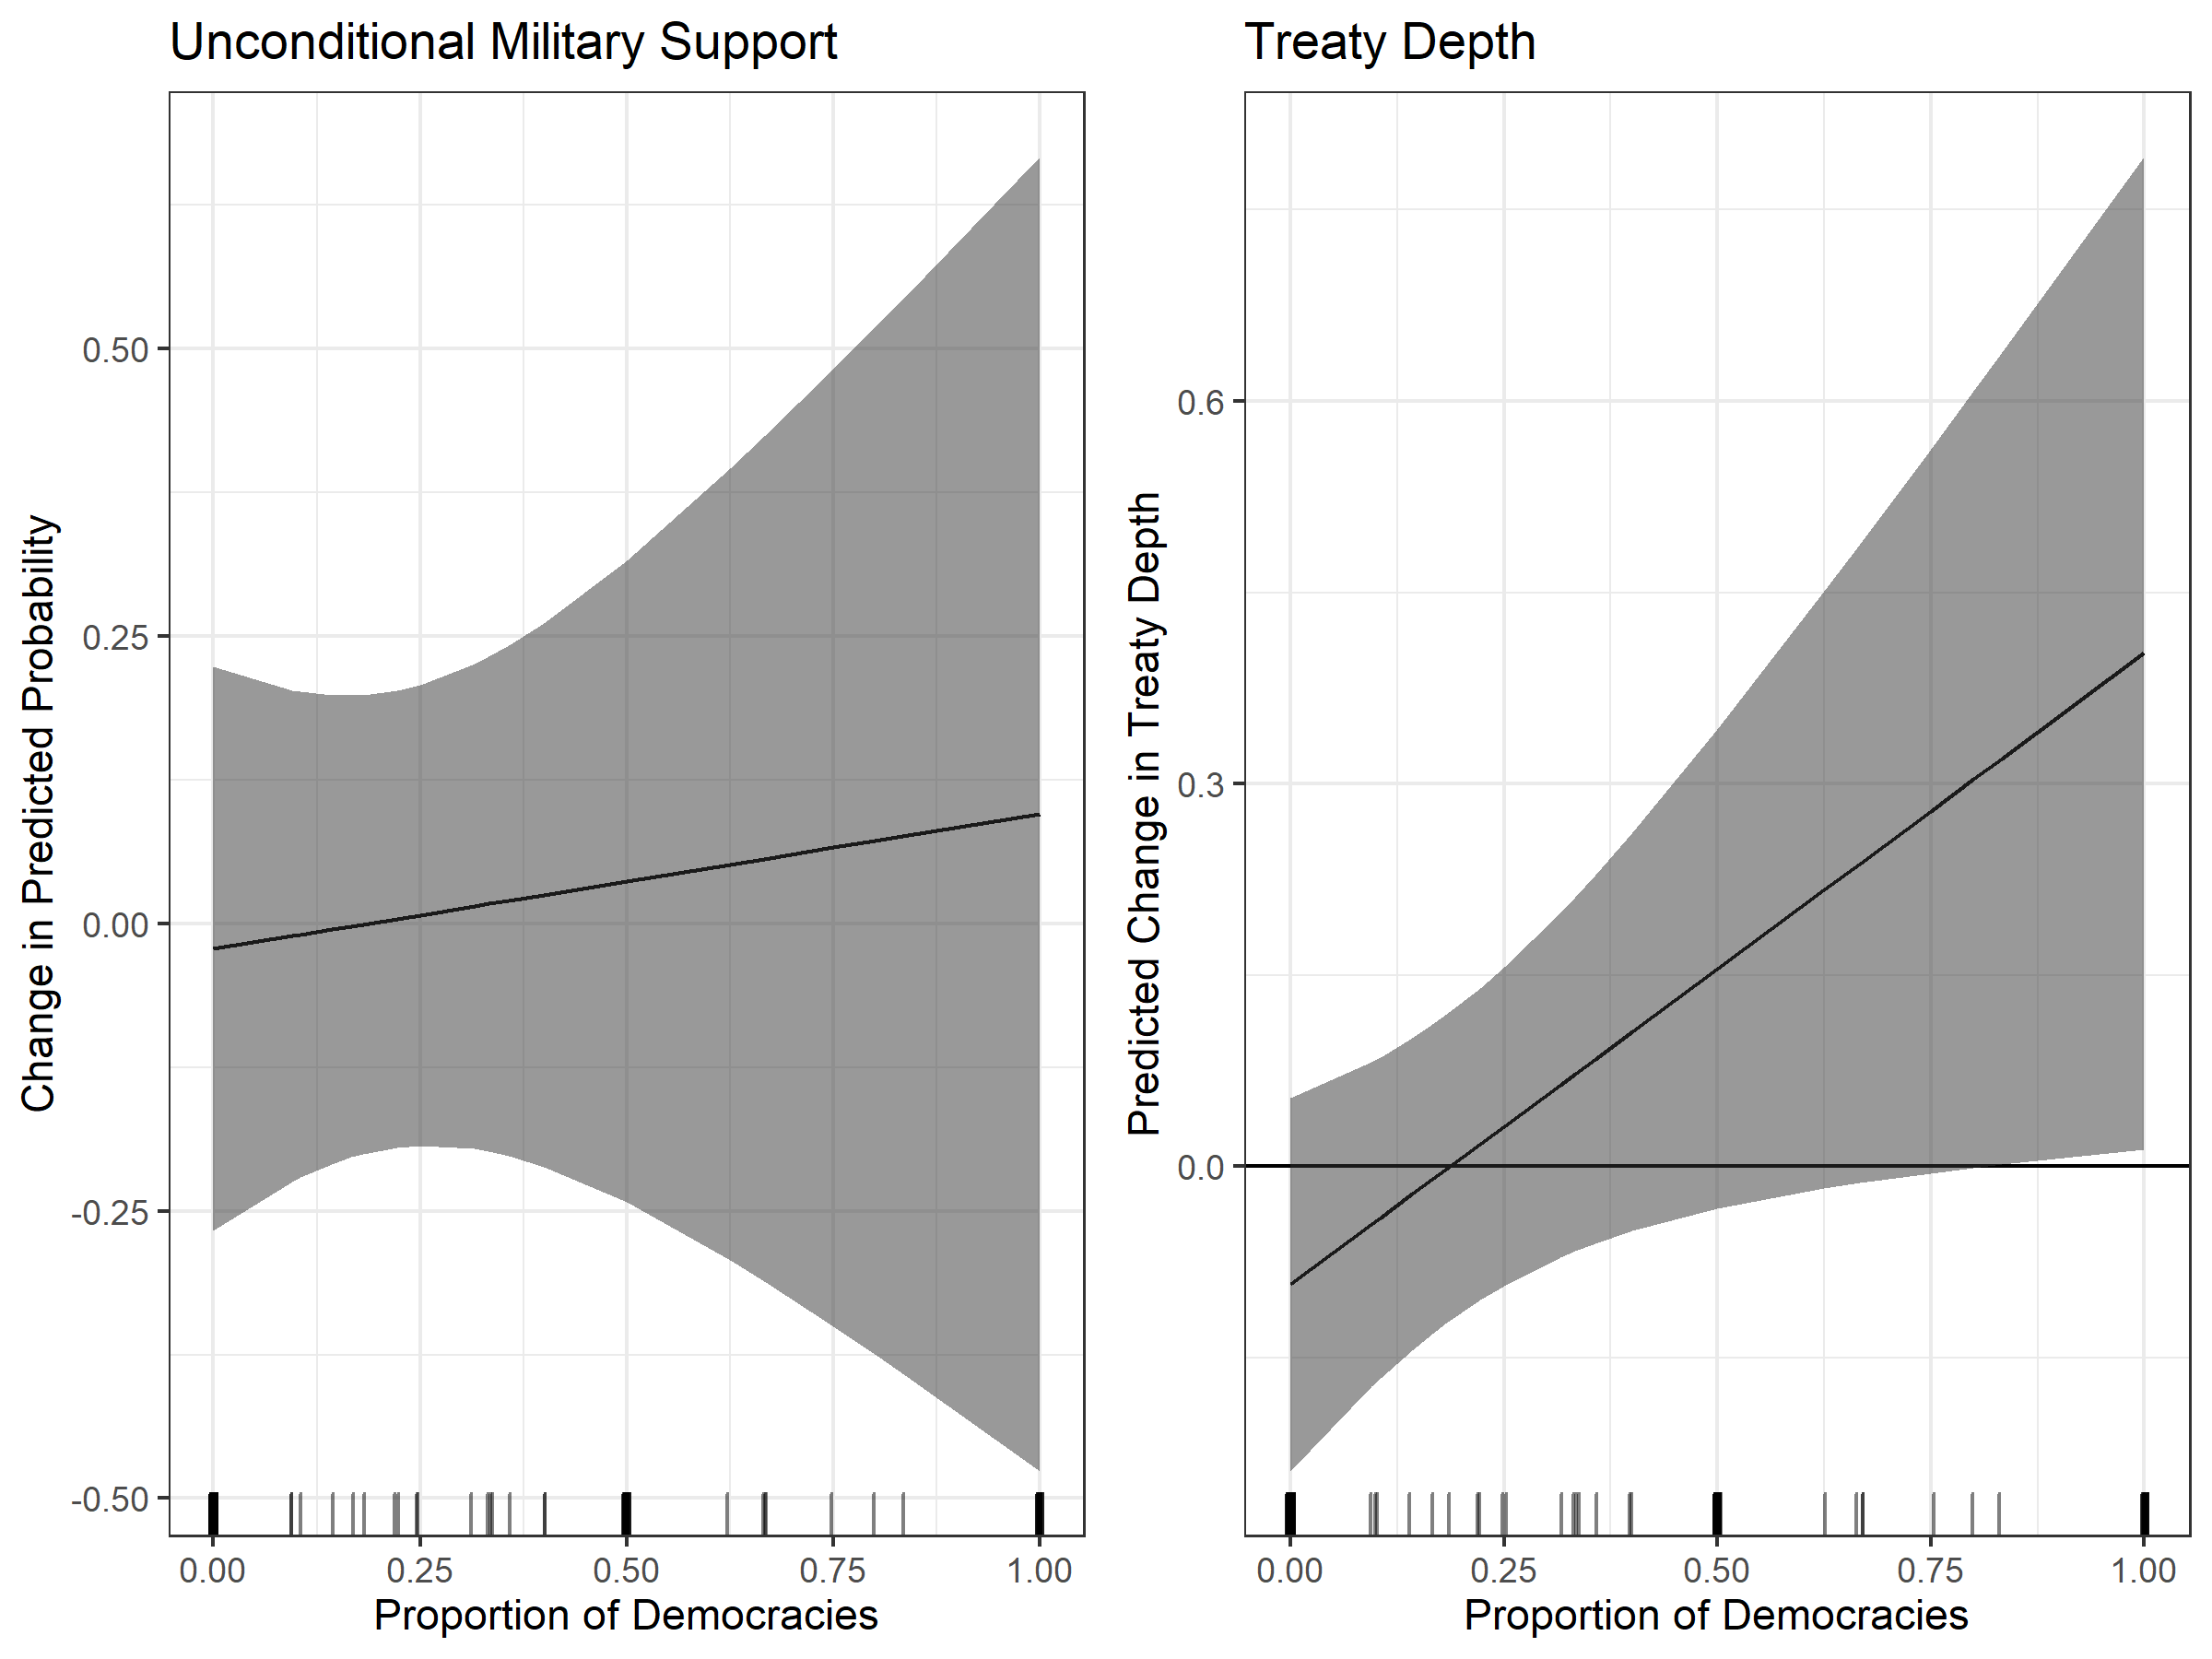
\includegraphics[width=.95\textwidth]{results-prop.png}  
\caption{Predicted probabilities of unconditional military support and predicted changes in treaty depth by the the proportion of democratic alliance members. The line marks predicted values, and the shaded areas encapsulate the standard errors. The rug plot on the x-axis marks observed values of allied democracy. Predictions based on the smoothed terms from the joint generalized regression model.}
\label{fig:results-prop}
\end{figure}



Differences between the joint and separate models of democratic proportion and alliance design are driven by correlations in the error terms of the depth and unconditional support models.  
Kendall's $\tau$ measures the strength of the correlation between the errors, and is a function of a parameter $\theta$ that I modeled in the third GJRM equation.
I used the start year of the alliance to predict differences in $\theta$, which affects correlations in unobservables between depth and unconditional military support. 
\autoref{fig:results-error} plots the smoothed term I used to predict the correlation in the error terms between treaty depth and unconditional military support. 
The predicted values in the top panel of \autoref{fig:results-error} are on the scale of $\theta$. 
In the bottom panel, I plot predicted $\tau$ values against the start year of the alliance. 


\begin{figure}[hbtp]
\centering
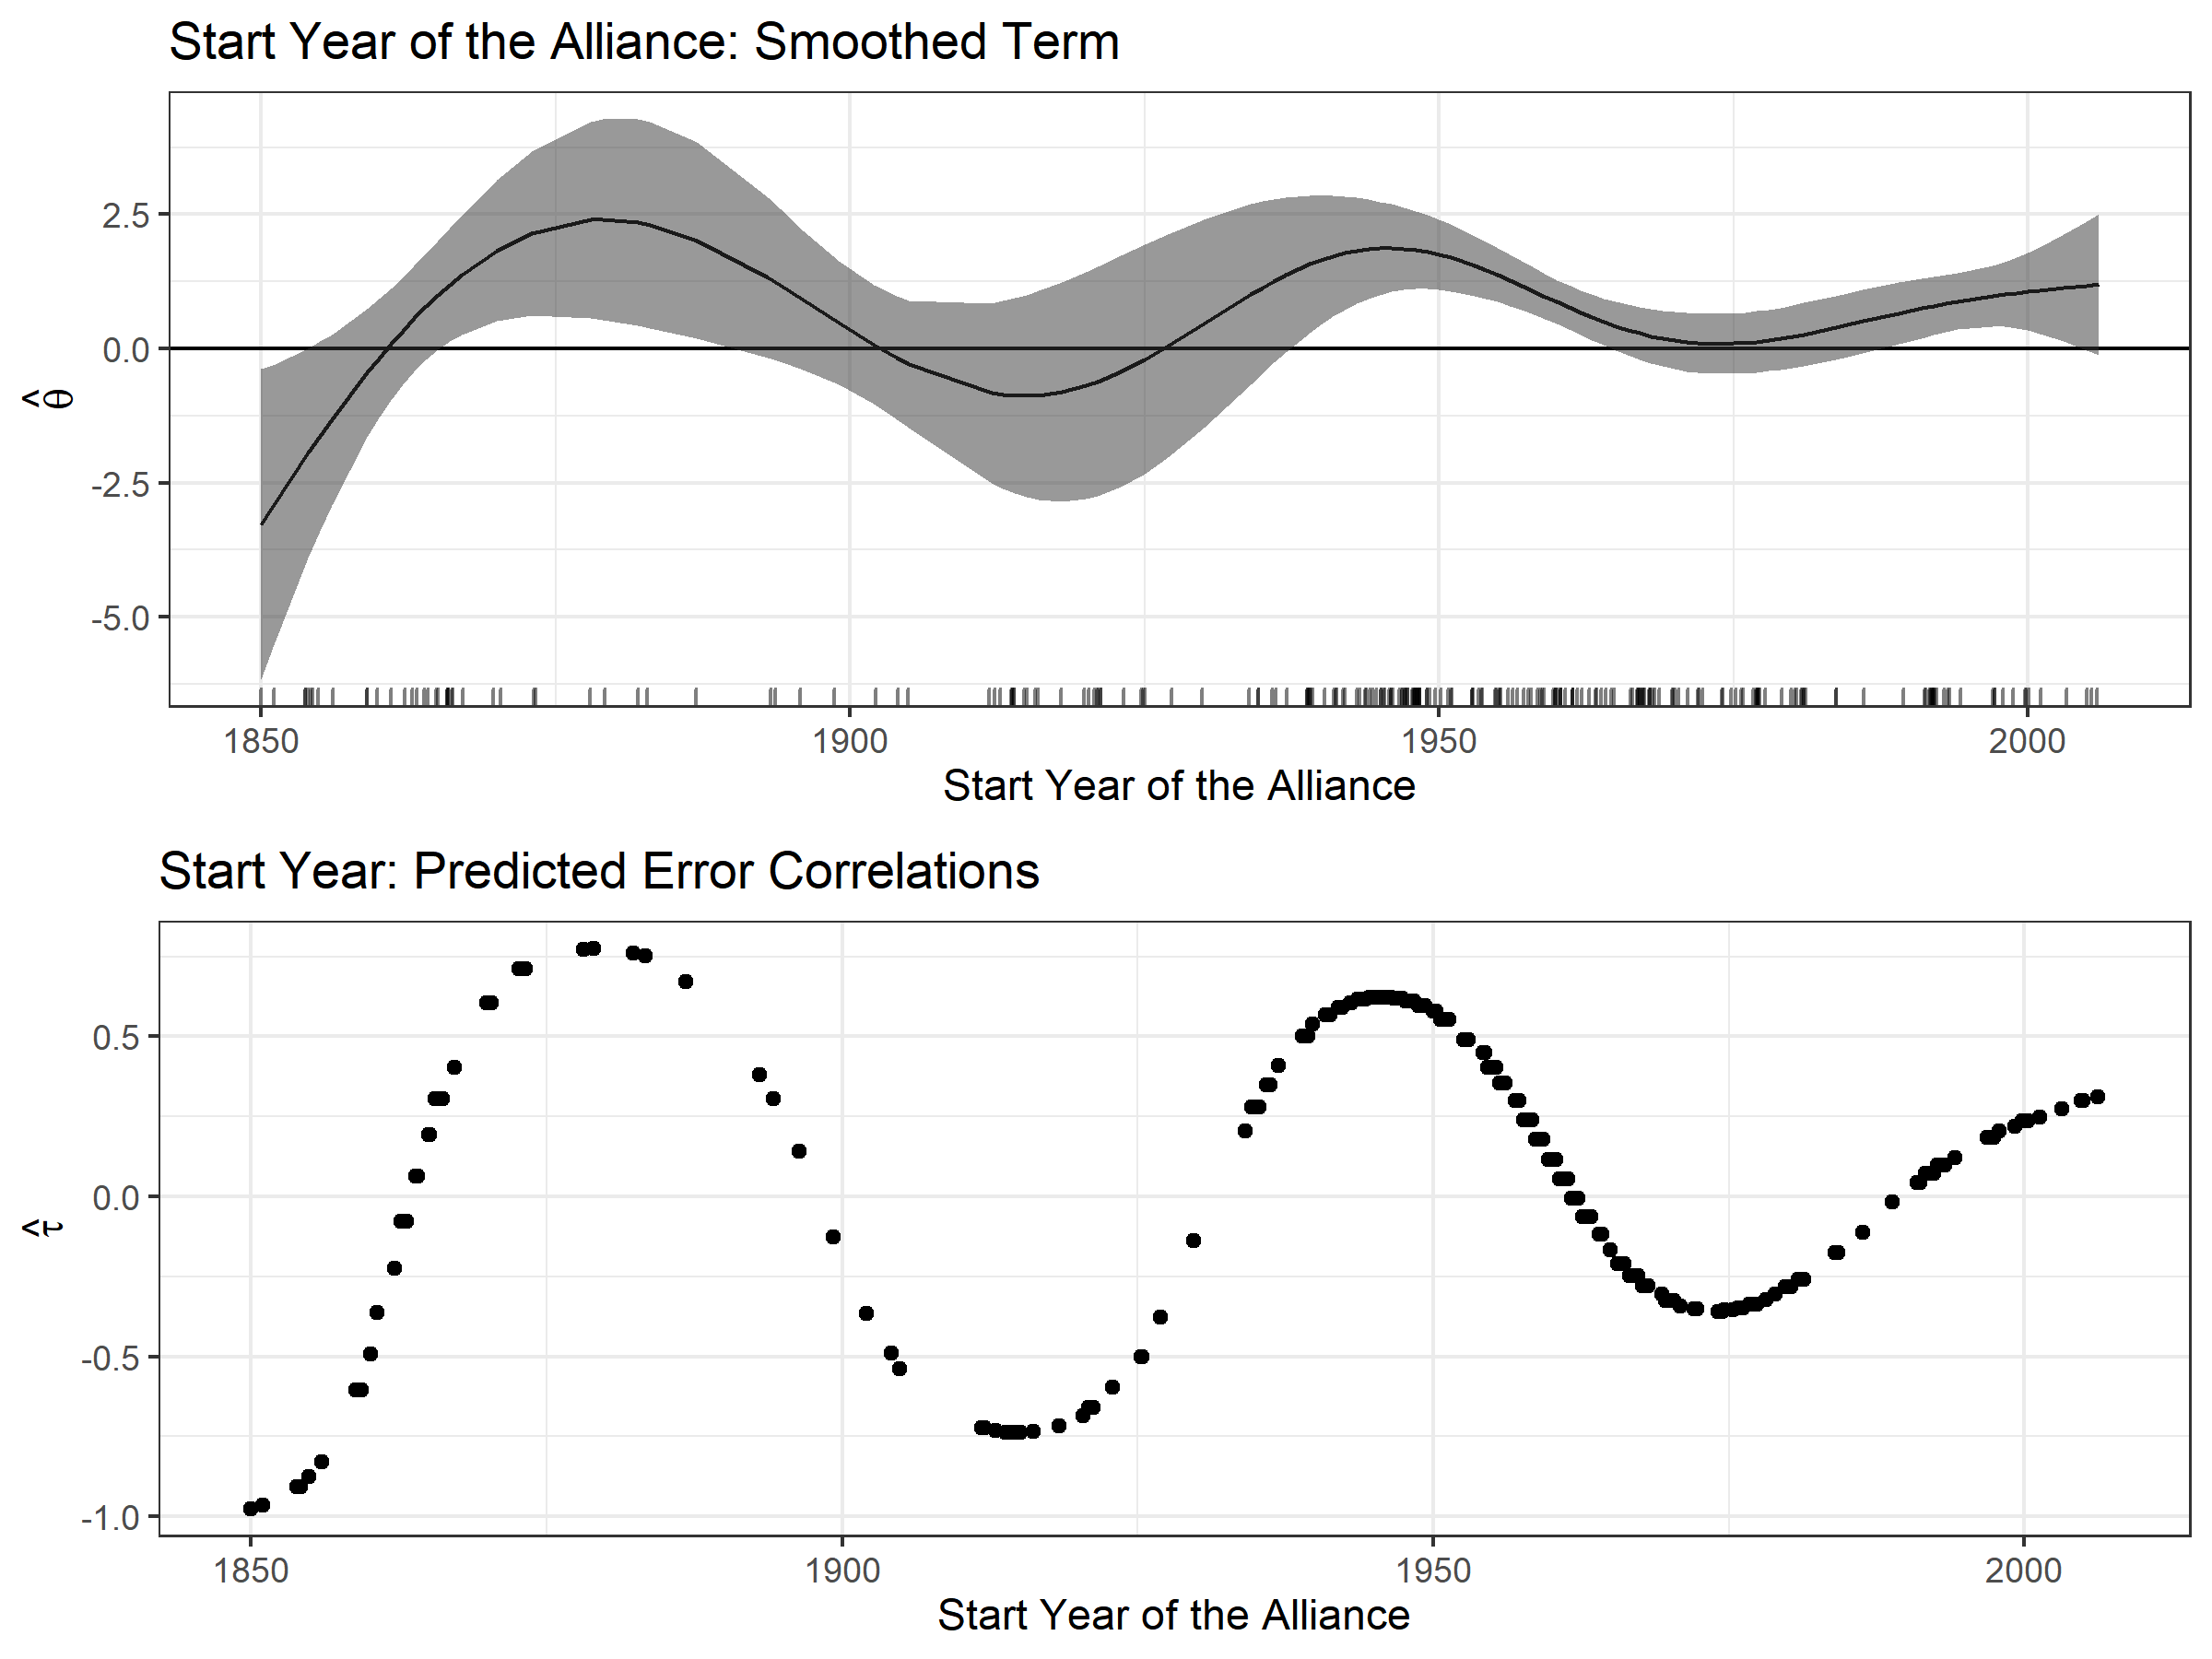
\includegraphics[width=0.95\textwidth]{../figures/results-error.png}
\caption{Predicted association between the errors of the unconditional military support and treaty depth equations in a generalized joint regression model by the start year of the alliance. There is limited alliance data before 1850, which dramatically increases uncertainty in the smoothed term. To make the plot more legible I present predictions from after 1850. The rug plot on the x-axis in the top row marks the distribution of alliances. Each point in the bottom row is an estimated $\tau$, one for each of the 277 observations.}
\label{fig:results-error}
\end{figure}


As \autoref{fig:results-error} shows, the association between the errors varies heavily by year. 
Most error correlations are positive between 1850 and 1900, before turning more negative between 1900 and 1950. 
During World War II depth and unconditional military support errors are positively associated. 
In general, the magnitude and direction of estimated correlation between depth and unconditional military support in unobserved factors $\tau$ changes dramatically over time.  


Again, correlations between unobserved factors are responsible for differences in results between the joint model and the separate models. 
After accounting for correlations in the error terms of the unconditional military support and treaty depth models, I find little connection between democracy and the probability of unconditional military support. 
Existing findings are sensitive to confounding from unobserved factors, which depth on shifts in the international context. 




\section{Alternative Measures of Treaty Depth}


There are two measures of treaty depth that operationalize similar concepts. 
\citet{LeedsAnac2005} develop an ordinal measure of military institutionalization.
\citet{BensonClinton2016} use a latent variable model to model treaty depth. 
While my measure is a better fit for my purposes in this paper, I find somewhat similar results with these two models. 
The null finding about unconditional military support holds. 
The Leeds and Anac measure of military institutionalization produces similar results in a GRJM model. 
The Benson and Clinton measure is harder to compare, because it covers fewer alliances and has more outliers that may impact inferences.


\autoref{fig:results-alt-measures} plots predictions from the average democracy smooth term for the two alternative measures. 
For the military institutionalization measure, I could not find an ordinal model in GJRM. 
Therefore, I created a dummy variable which is equal to one if the alliance had an institutionalization score of 1 or 2. 
I then modeled the military institutionalization dummy with a probit distribution. 
The results of this analysis match the treaty depth hypothesis, as the probability of military institutionalization is increasing in average democracy. 


\begin{figure}
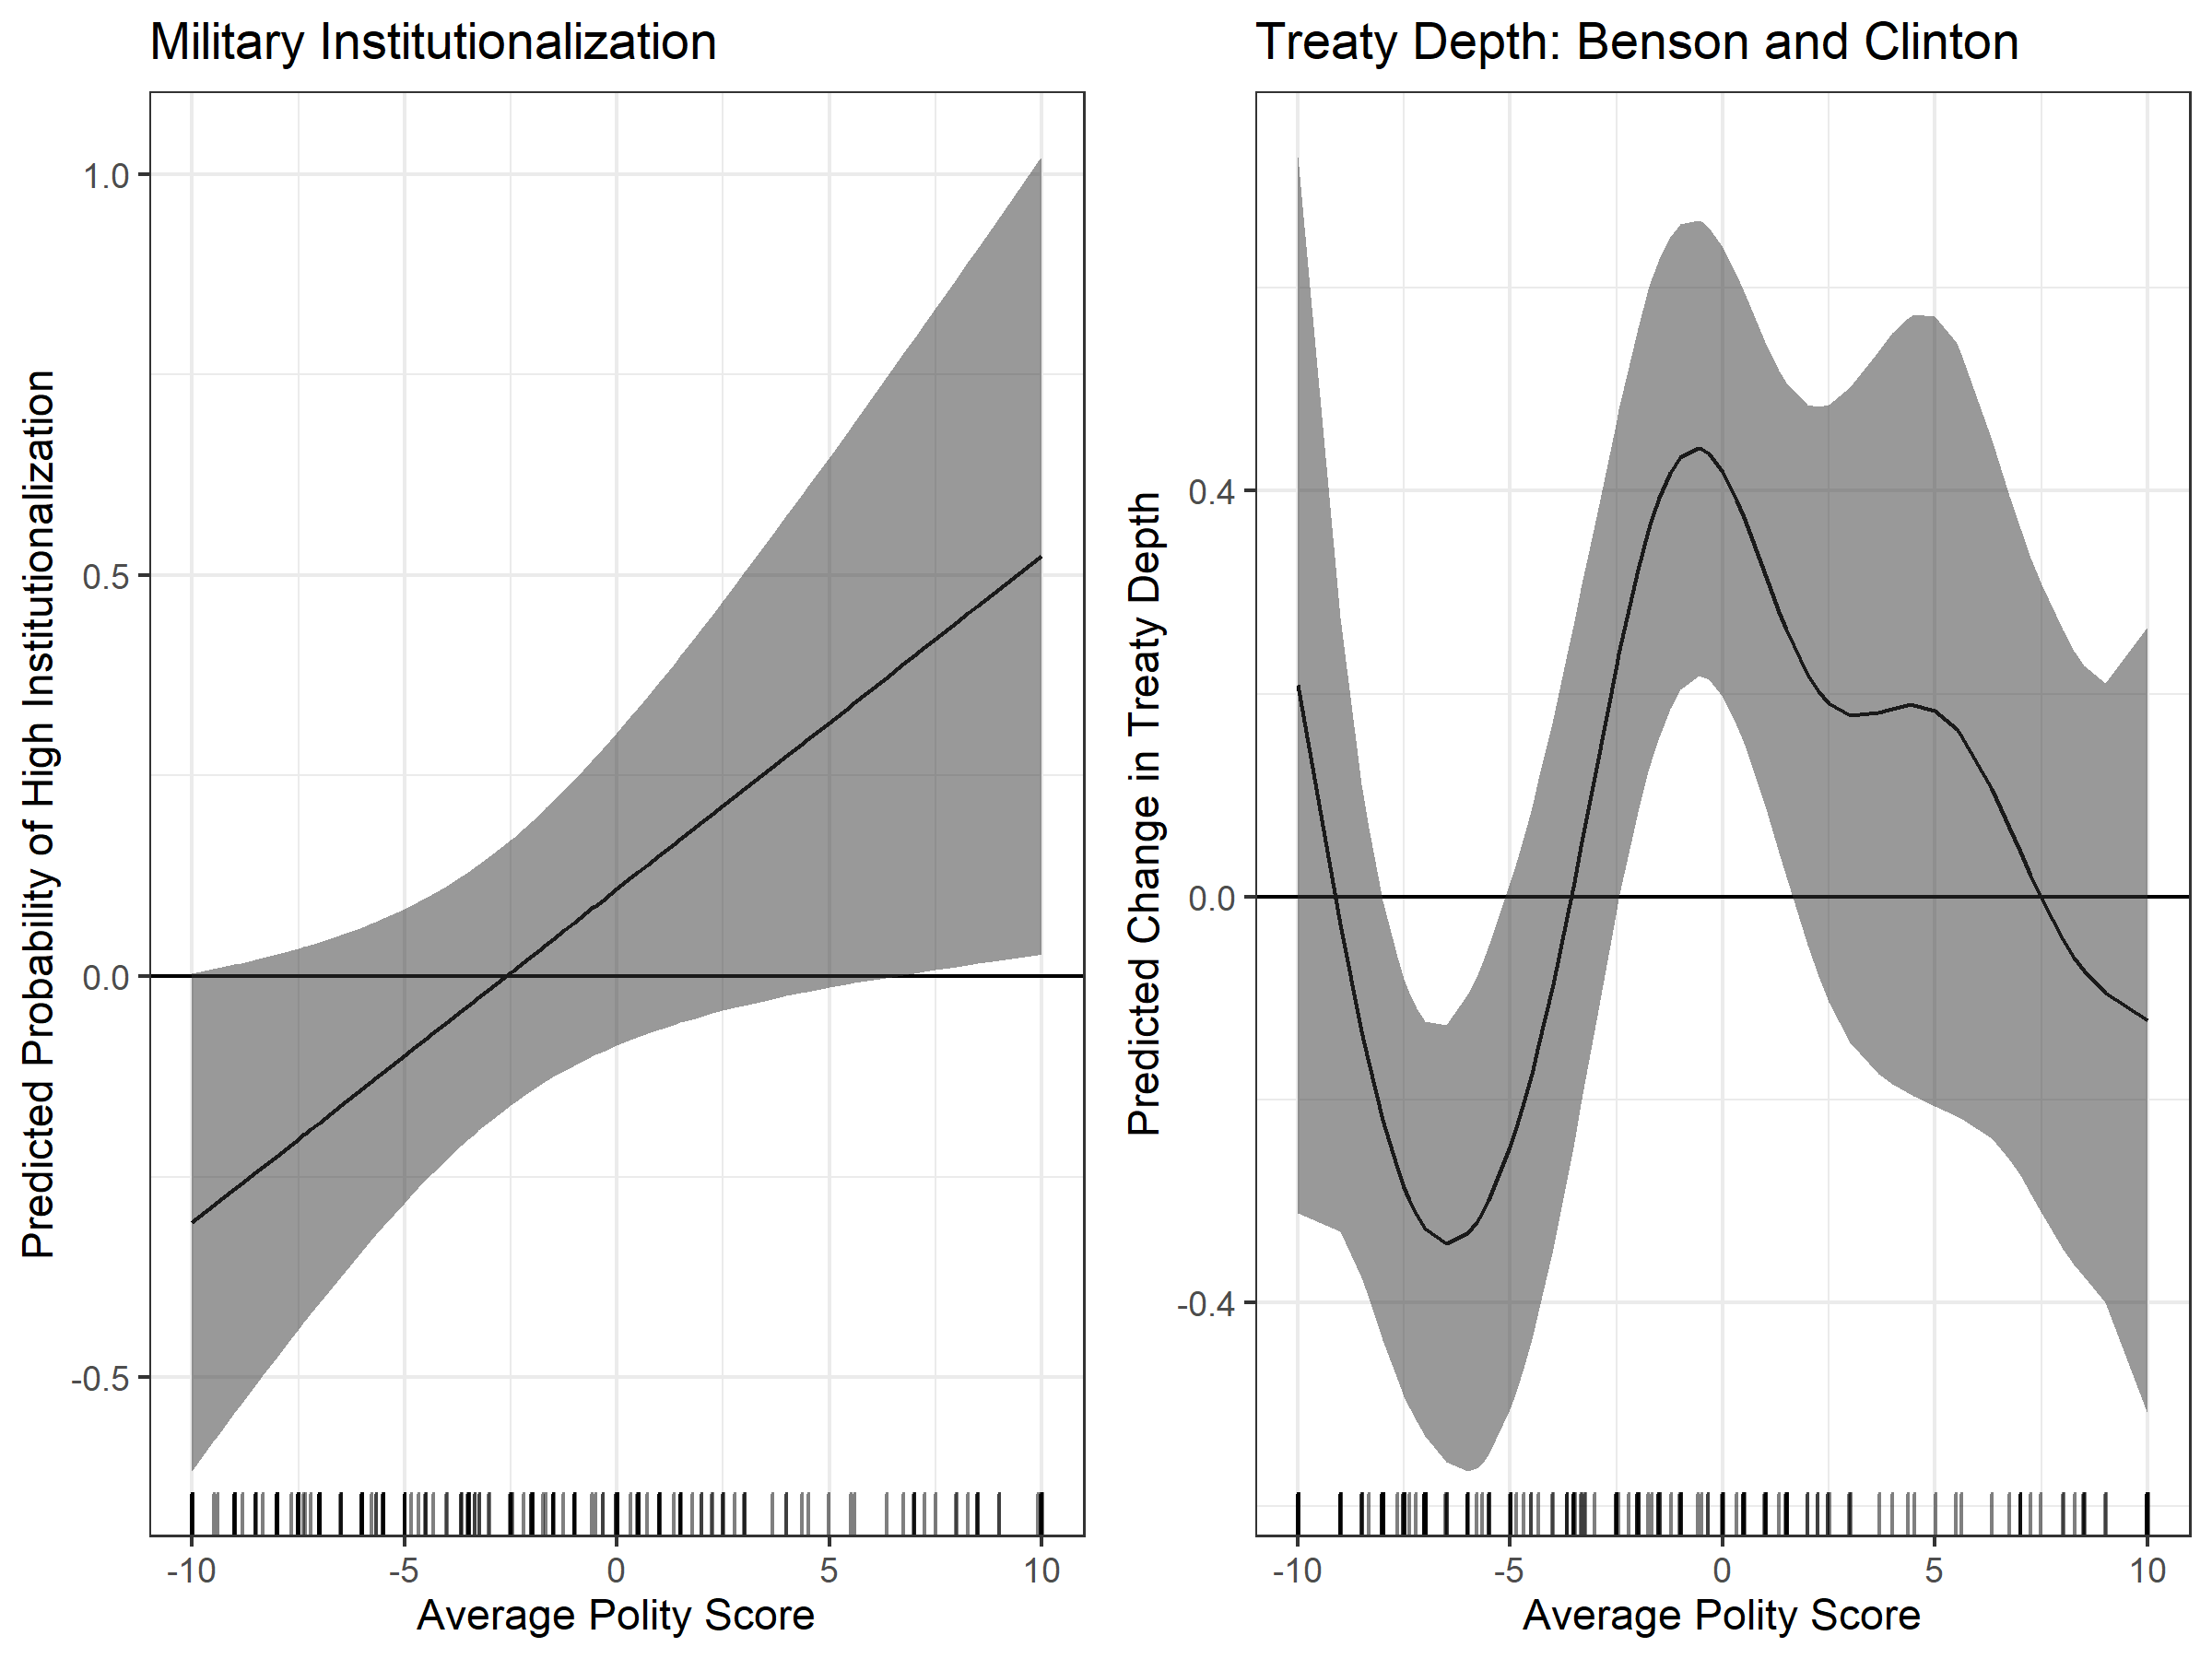
\includegraphics[width=.95\textwidth]{results-alt-measures.png}  
\caption{Predicted probabilities of unconditional military support and predicted changes in treaty depth by the the proportion of democratic alliance members. The line marks predicted values, and the shaded areas encapsulate the standard errors. The rug plot on the x-axis marks observed values of allied democracy. Predictions based on the smoothed terms from the joint generalized regression model.}
\label{fig:results-alt-measures}
\end{figure}

Findings about the association between treaty depth and Benson and Clinton's measure are more mixed. 
The relationship is highly non-linear, and high average democracy is not positively correlated with Benson and Clinton's measure of depth. 



\section{Adjusting for Alliance Formation}


Observed alliances are the result of negotiations between potential members. 
Some alliance negotiations fail, however, so the set of observed alliances is not a random sample \citep{Poast2019a}. 
In this section, I account for alliance formation, and show that a hurdle model of alliance treaty depth and conditions on military support produces similar inferences. 


My research design for this robustness check follows existing procedures for dealing with selection into alliances and treaty design. 
To construct the dataset, I followed the process of \citet{Poast2010} for dealing with k-adic data, because alliances can have more than two members. 
First I constructed a random sample of groups of states that could have formed an alliance in each year, but did not \citep{FordhamPoast2014}.
I then took a stratified sample of the non-allied k-ads to include five times as many non-allied observations as alliance observations for each observed value of alliance size. 
For example, there are 215 bilateral alliances, so I included 1075 non-allied bilateral groups. 
There is only one alliance with 34 members, so I include five non-alled k-ads with 34 members. 
Finally, I summarized the characteristics of these non-allied k-ads and merged them with the observed alliance data. 


To model this process, I built on the research design of \citet{Chibaetal2015}. 
They used a hurdle model to assess whether after accounting for non-random selection into alliances, democracies were more likely to offer conditional obligations.
Hurdle models have two stages or parts.
A first stage model predicts which observations clear the hurdle to a second stage where the outcome is observed. 
Unlike a sample selection model, the second stage in a hurdle model is logically undefined, which is how alliance treaty design works.\footnote{Hurdle models also do not require an exclusion restriction.} 
After overcoming the barriers to alliance formation, states then specify treaty content. 


Unlike \citet{Chibaetal2015} 
Therefore, I jointly estimate two hurdle models- one for the depth and the other for unconditional military support. 
To have zero values for the outcome at the hurdle stage, I adjusted the outcomes in these models. 
First, I rescaled latent depth by adding one, which shifted the distribution onto uniformly positive values. 
I then applied a gamma hurdle model to this shifted depth outcome and used the same covariates as the main model in the manuscript to predict depth. 
For unconditional military support, I replaced the dummy indicator in the manuscript with an ordinal indicator.
This ordinal variable is captures the relative strength of the military support promise in the alliance. 
ATOP alliances can be conditional on four things: adversaries, locations, a particular conflict, the number of opponents, a specific demand or non-provocation in the case of defense treaties. 
The maximum number of observed conditions in an alliance is four, which is the most conditional and limited alliance in the data. 
I therefore invert the number of conditions and assign unconditional alliances a value of four. 
Essentially, the measure then captures the number of circumstances where an alliance could have applied conditions but did not. 
To avoid including zeros in the measure, I add one to it, because promising military support adds some baseline strength to any alliance \citep{Morrow2000}. 
Thus, the final measure of military support commitment strength ranges between 1 and 5 for observed alliances, but is zero for non-alliances. 
In both models, I use average democracy, mean threat, asymmetric capability and wartime variables in the hurdle equation. 


I then estimate the two hurdle models simultaneously using the BRMS package for R, which employs STAN for fully Bayesian inference \citep{Buerkner2017}. 
Unlike the GJRM models in the manuscripts, there is no correlation between the residuals of the separate hurdle models, but Instead, I connect the two models with a correlated set of year varying intercepts. 
The complexity of this joint hurdle model and limited sample size in the second stage means results should be treated with caution.\footnote{I do find similar results with separate hurdle models for depth and conditions on military support.} 


Even after accounting for non-random alliance formation with the joint hurdle model, I find similar results to the appendix. 
\autoref{fig:results-prop} plots the results of the joint hurdle model. 
As in the sample with only observed alliances, greater democracy among alliance members has no clear relationship with conditionality, but increases treaty depth. 


\begin{figure}
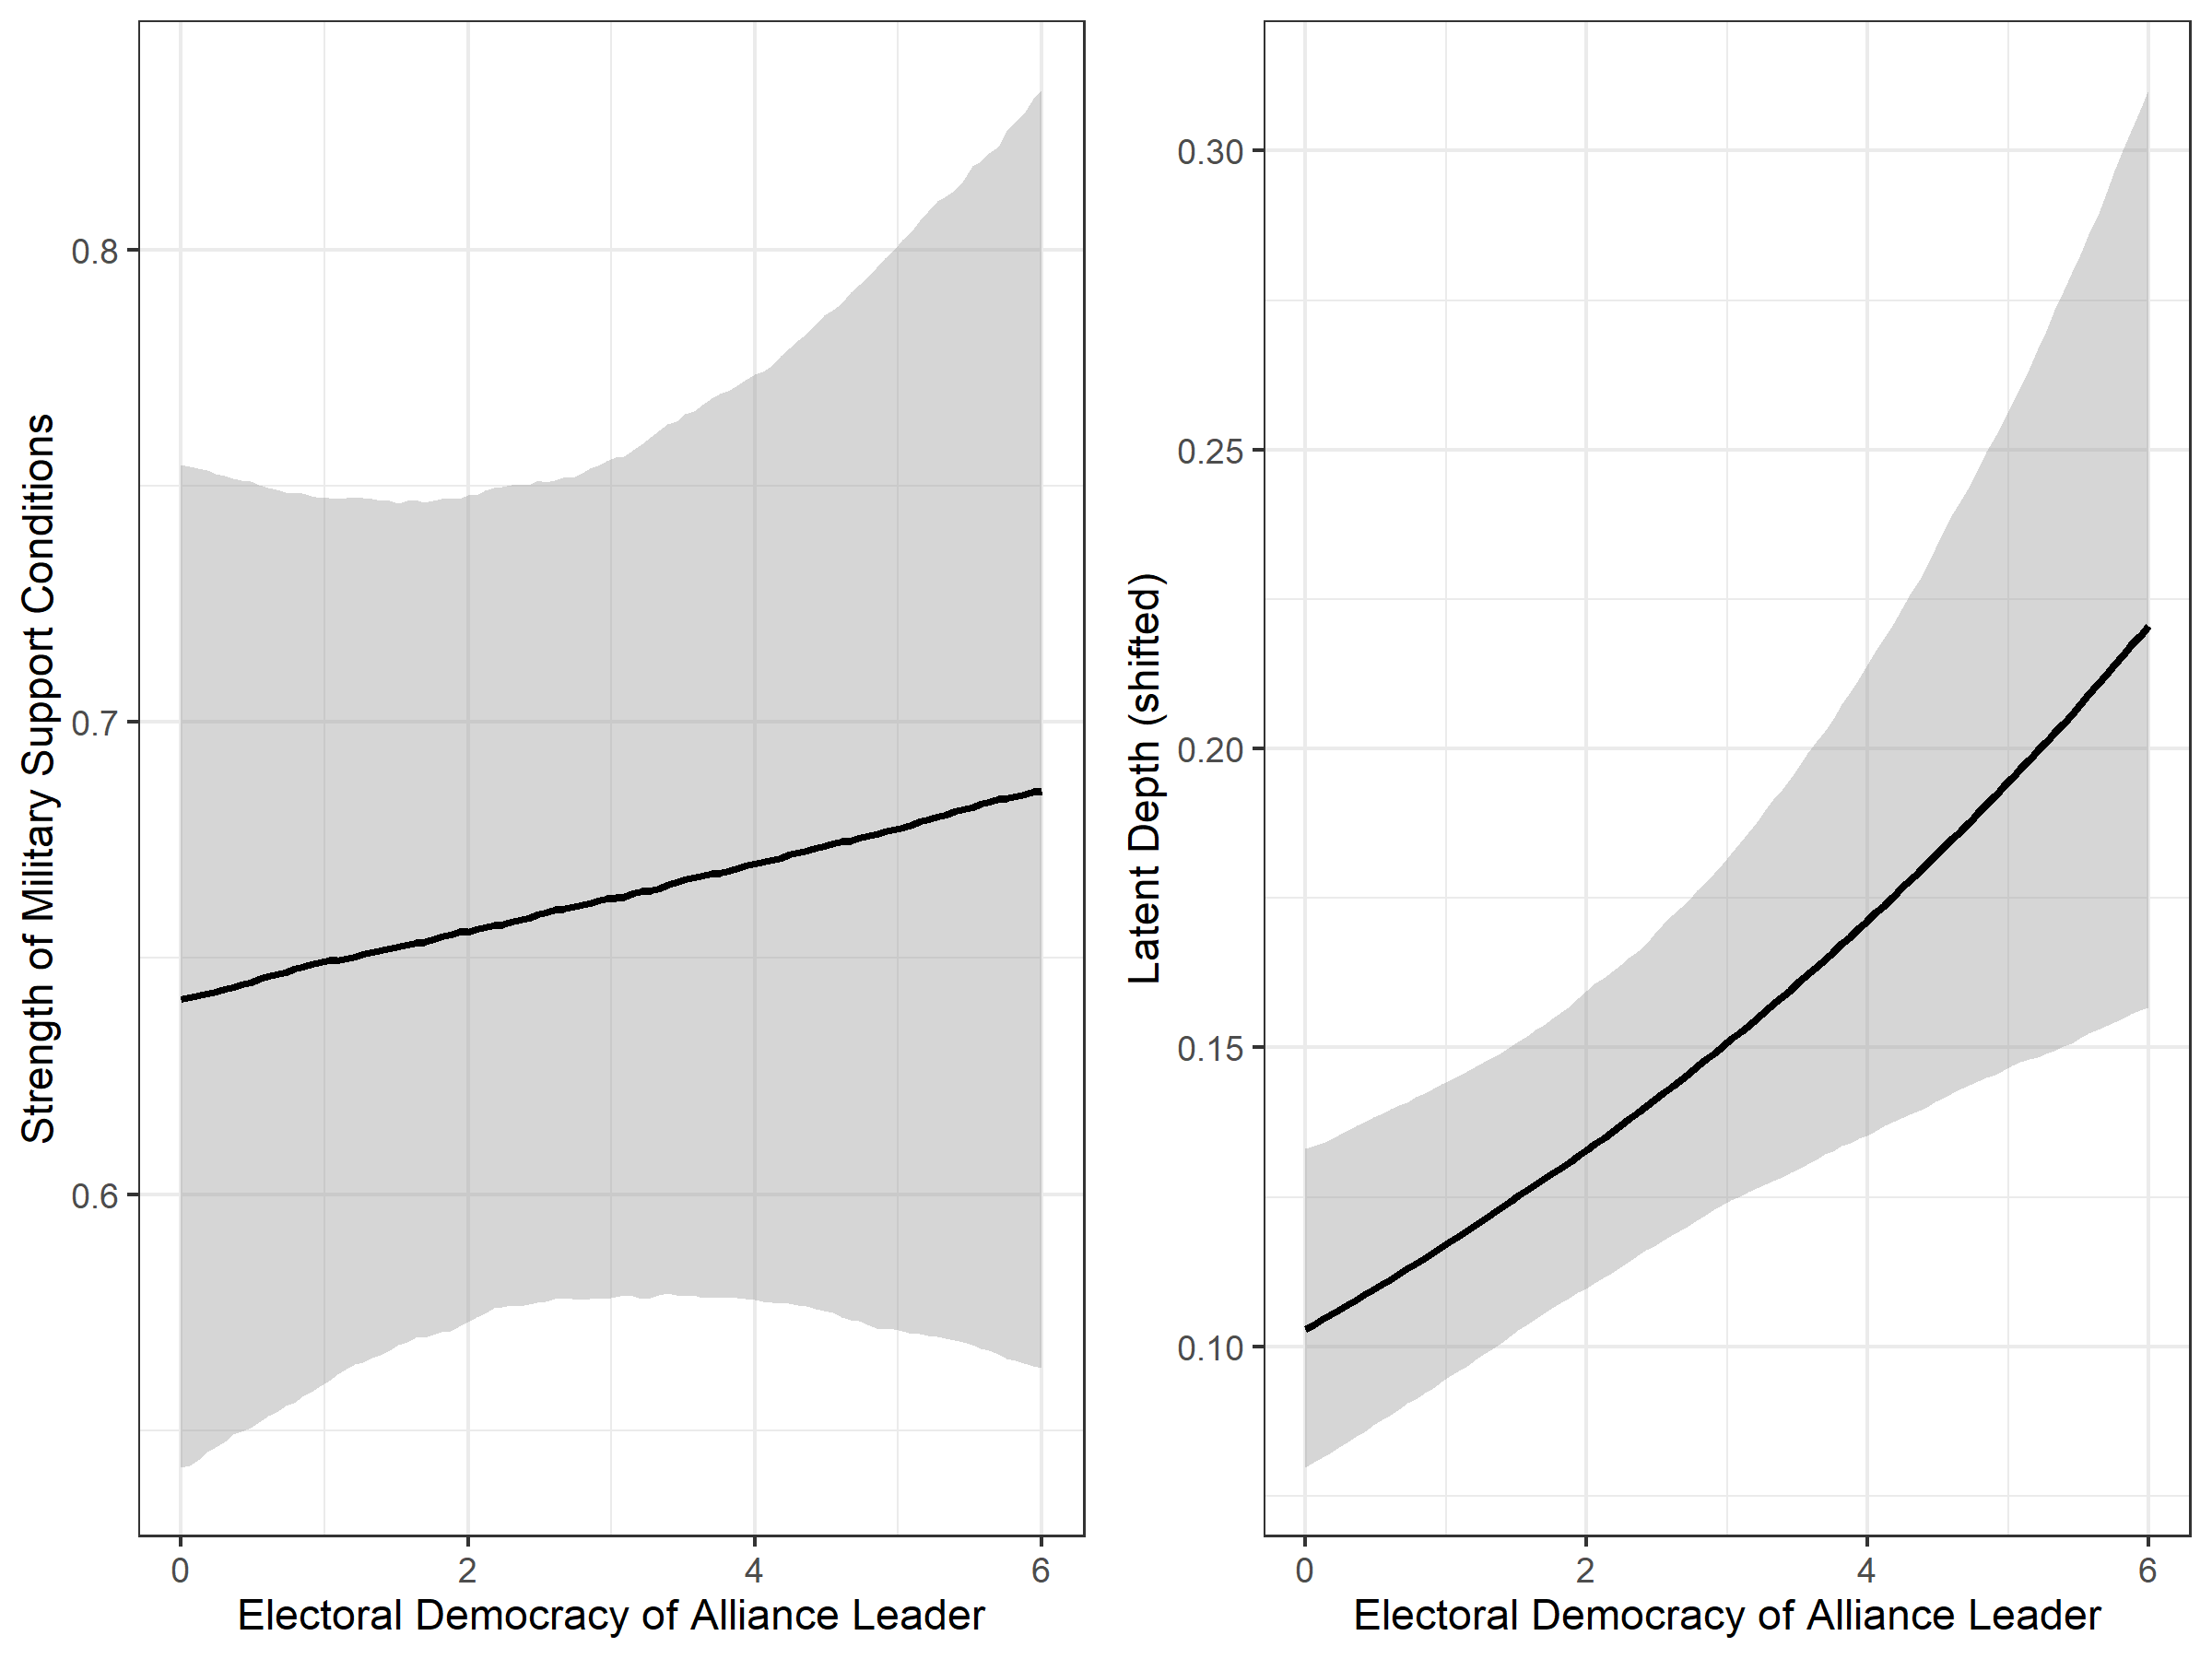
\includegraphics[width=.95\textwidth]{results-joint-hurdle.png}  
\caption{Predicted strength and predicted changes in treaty depth by the the average POLITY score alliance members when the treaty formed based on a joint hurdle model of alliances. The line marks predicted values, and the shaded areas encapsulate the 90\% credible interval. The rug plot on the x-axis marks observed values of allied democracy. Predictions holding all other variables.}
\label{fig:results-joint-hurdle}
\end{figure}





\section{Uncertainty in Latent Treaty Depth} 


In a separate model, I consider how measurement uncertainty shapes inferences about the connection between non-major power alliances and treaty depth. 
The latent measure of treaty depth has some uncertainty. 
This is a reasonable approximation of alliance politics, because alliance treaty depth is not observed with certainty. 
There are perceptible differences in treaty depth, especially once states add substantial depth to the treaty. 
Even so, the results from the analysis of mean treaty depth may overstate the effect of non-major power membership. 


To incorporate uncertainty over treaty depth, I fit a modification of the joint model. 
First, I created 1,000 datasets, one for each draw of the posterior distribution of the latent measure.
Then I fit the model of mean treaty depth to 500 randomly sampled datasets from those 1,000 to facilitate computation. 
For models of depth with uncertainty, I use BRMS \citep{Buerkner2017}. 
BRMS is an interface to STAN, a probabilistic programming language for Bayesian estimation \citep{Carpenteretal2016}. 
Joint Bayesian estimation has the flexibility to incorporate the probit and beta models and can be easily extended to account for uncertainty in the depth measure, but it does not allow correlated errors. 
Fitting the model sequentially to each dataset produces 500 separate models, which I combine into a single model by aggregating the posterior draws in a single posterior that accounts for uncertainty in the treaty depth measure.\footnote{Standard convergence diagnostics indicate convergence in all 500 models. Diagnostics like $\hat{r}$ are less useful for the full posterior, because some of the chains in the submodels do not overlap.}
This approach is analogous to common techniques for analyzing missing data, where multiple imputation generates uncertainty about the missing values \citep{Hollenbachetal2018imp}.
After multiple imputation, researchers fit a separate model to each imputed dataset and then combine the results. 


% Expand on these results later 
After accounting for uncertainty over treaty depth, I find a similar pattern. 
Allied democracy increases treaty depth, but decreases the probability of unconditional military support. 


\singlespace
 
\bibliography{../../../MasterBibliography} 





\end{document}